\chapter{Background}
\label{chap:background}

This chapter presents the conceptual and methodological foundations required to understand the proposed research on enhancing computational efficiency in multi-temporal building change detection. Section~\ref{sec:sat-imagery} introduces the fundamentals of satellite imagery and resolutions relevant to Very High Resolution (VHR) analysis (e.g., PeruSAT-1). Section~\ref{sec:bcd-prelim} formalizes the building change detection (BCD) problem and its urban challenges in Latin America. Section~\ref{sec:transformers-attn} reviews Transformer backbones and attention mechanisms, starting from standard (softmax) self-attention and advancing to linear and low-rank attention---with emphasis on the Reduced-Rank Linear Attention (RALA) formulation integrated later into ChangeFormer. Section~\ref{sec:metrics} describes evaluation metrics. Section~\ref{sec:bg-final} outlines the final considerations linking these foundations to our RALA-ChangeFormer proposal.

\section{Satellite Imagery Concepts}
\label{sec:sat-imagery}

Satellite imagery is one of the primary sources of information for monitoring the Earth’s surface. These images are obtained from sensors installed on artificial satellites orbiting the planet, which capture electromagnetic radiation reflected or emitted by objects across different wavelengths. Depending on the type of sensor, it is possible to record bands in the visible spectrum, near-infrared, thermal infrared, or microwave domains, enabling a wide range of applications from agriculture to urban planning.\footnote{Raya-Armenta, J. M., et al. (2021). A short review of radiation-induced degradation of III–V photovoltaic cells for space applications. \textit{Solar Energy Materials and Solar Cells}, 233, 111379. doi: \url{https://doi.org/10.1016/j.solmat.2021.111379}}

\begin{figure}[h!]
    \centering
    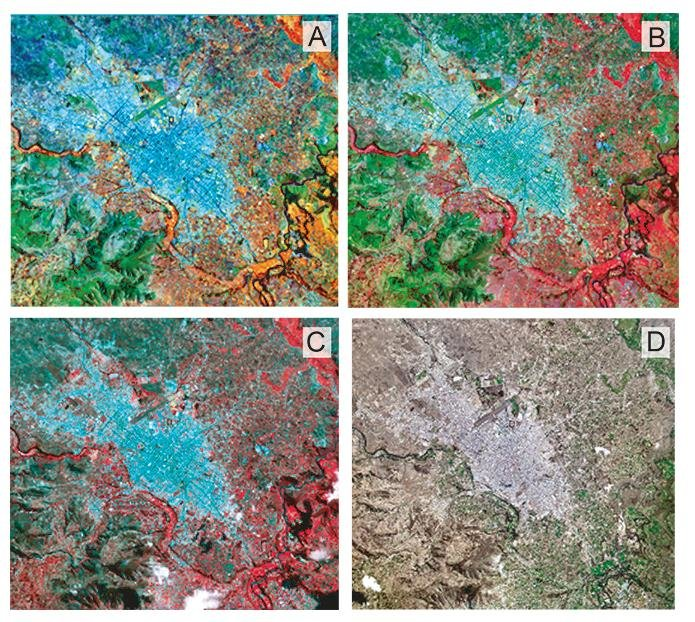
\includegraphics[width=0.6\textwidth]{graficos/imgs-satelitales.jpg}
    \caption{Sample of the same scene observed across different satellite bands.}
    \label{fig:imgs-satelitales}
\end{figure}

\newpage

\subsection{Types of satellites according to their orbit}
Earth observation satellites can be broadly classified according to their orbit. This parameter determines their altitude, coverage, and revisit frequency, conditioning the type of applications for which they are suitable.

\noindent \textbf{Geostationary Orbit satellites (GEO).} Located at an altitude of approximately 36,000 km above the equator, geostationary satellites maintain a fixed position relative to a point on Earth’s surface. This makes them suitable for meteorological and telecommunications applications, as they provide continuous monitoring of large portions of the planet. However, their great distance limits the achievable spatial resolution, making them less adequate for detailed urban studies.

\noindent \textbf{Low Earth Orbit satellites (LEO).} Low Earth Orbit (LEO) satellites, situated between roughly 700 and 2,000 km in altitude, perform several passes per day over the same region. Due to their proximity to Earth, they can capture imagery with high spatial resolution, which makes them the main source for terrestrial observation applications, including agricultural, environmental, and urban monitoring. This category includes very high-resolution (VHR) satellites such as PeruSAT-1, capable of capturing details up to 0.70 m per pixel (panchromatic resolution),\footnote{PeruSAT-1 technical specifications: panchromatic resolution $\sim$0.70 m, multispectral resolution $\sim$2.8 m. See Airbus PeruSAT-1 datasheet; EO Portal; N2YO.} which are essential for the analysis of individual buildings.

\begin{figure}[h!]
    \centering
    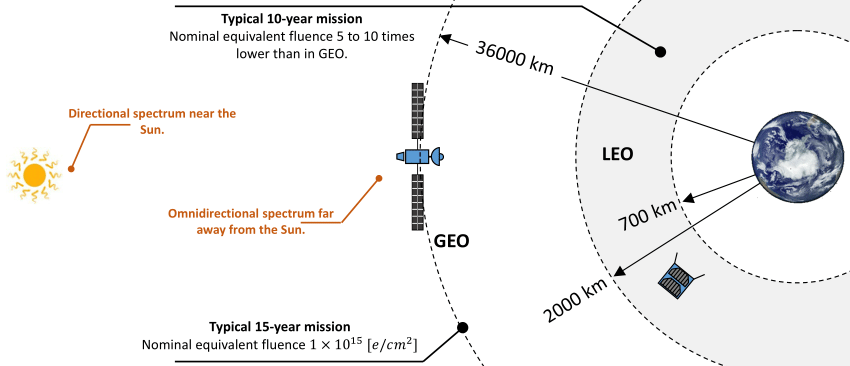
\includegraphics[width=0.6\textwidth]{graficos/GEOvsLEO.png}
    \caption{Comparison between Geostationary Orbit (GEO) and Low Earth Orbit (LEO) satellites.}
    \label{fig:GEOvsLEO}
\end{figure}

\subsection{Resolution in satellite images}

The quality and applicability of satellite imagery does not depend only on the type of orbit, but also on its resolutions.\footnote{Introduction to Remote Sensing. \url{https://eol.pages.cms.hu-berlin.de/geo_rs/S02_image-prop1.html}} These can be grouped into four main dimensions:

\begin{itemize}
    \item \textbf{Spatial resolution}: pixel size on the ground, determining the level of observable detail.
    \item \textbf{Spectral resolution}: number and width of recorded bands, enabling the discrimination of different materials or land covers.
    \item \textbf{Radiometric resolution}: sensor sensitivity to distinguish intensity levels within each band.
    \item \textbf{Temporal resolution}: frequency with which the satellite revisits the same area, fundamental for multi-temporal studies.
\end{itemize}

\begin{figure}[h!]
    \centering
    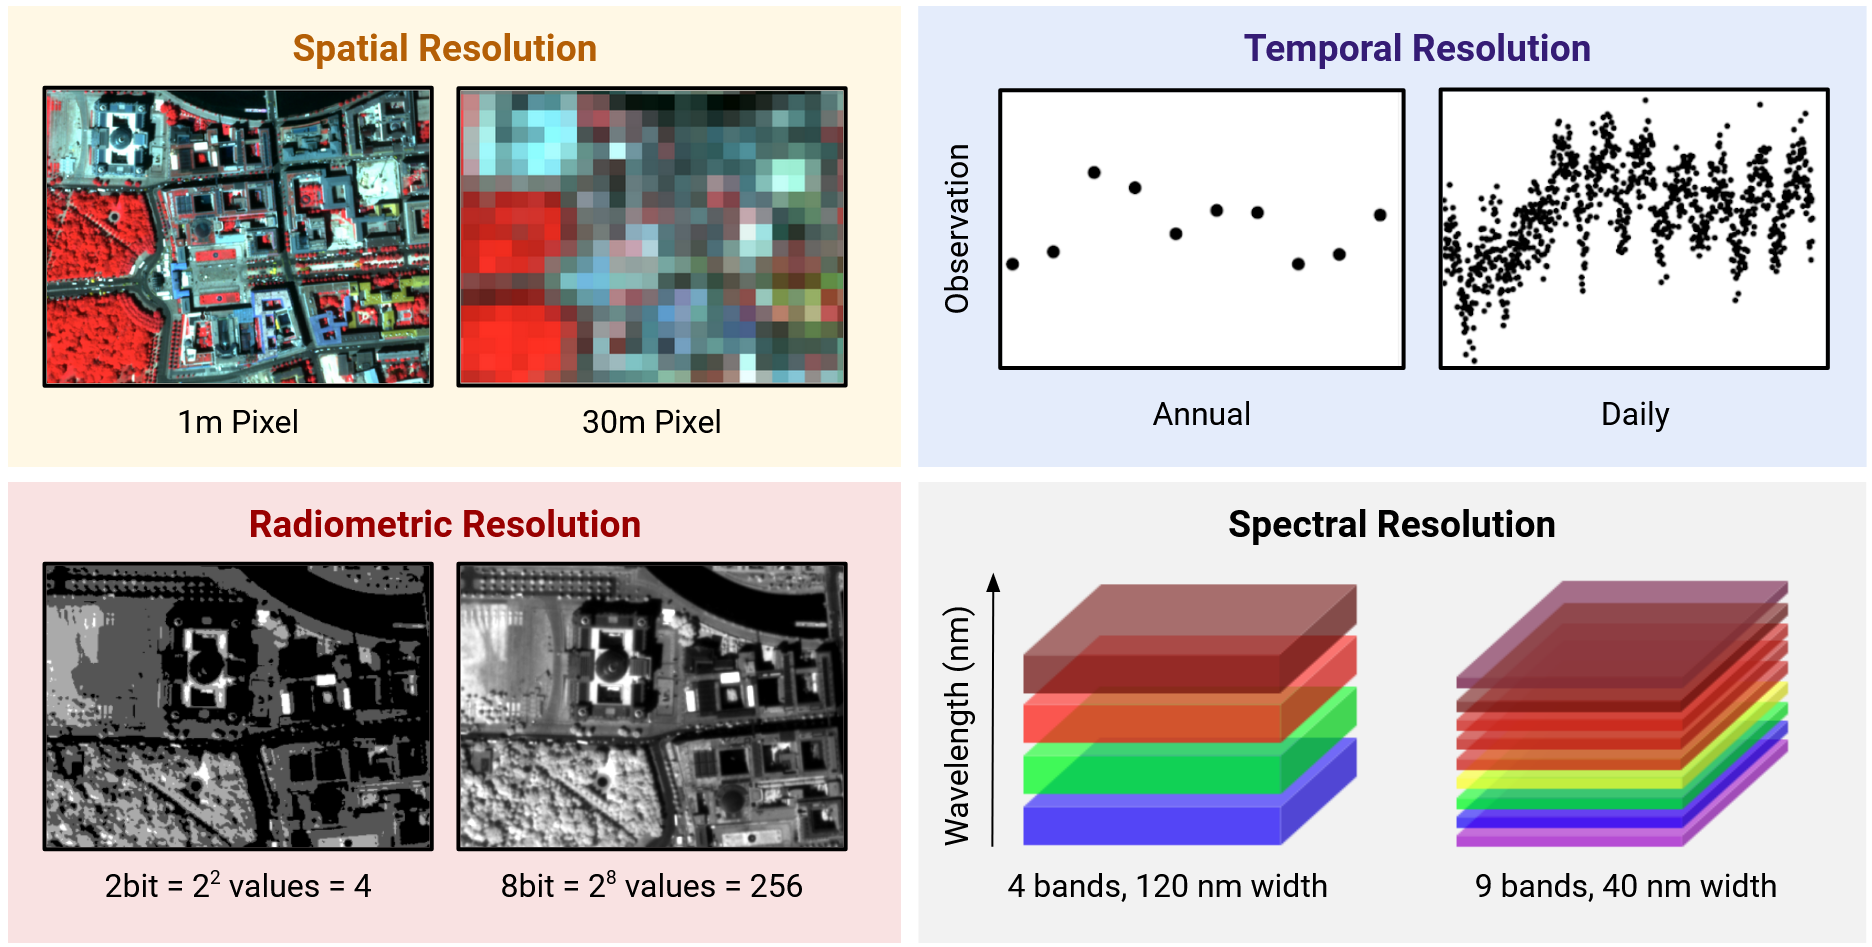
\includegraphics[width=0.6\textwidth]{graficos/resolutions.png}
    \caption{Satellite image resolutions relevant to urban analysis.}
    \label{fig:resolutions}
\end{figure}

\section{Building Change Detection Preliminaries}
\label{sec:bcd-prelim}

How can changes in the urban fabric of Lima be automatically detected over time? What is the difference between horizontal expansion—when new land is occupied—and vertical densification—when buildings increase in height? From a computational point of view, multitemporal change detection aims to identify and classify variations in building footprints or structures by comparing satellite imagery captured at different moments. This task, known as building change detection (BCD), provides critical insights for urban planning, infrastructure management, and risk assessment. Therefore, in this section, we provide a general introduction to the problem, its challenges, the types of changes considered, and the main methodological approaches.

\begin{figure}[h!]
    \centering
    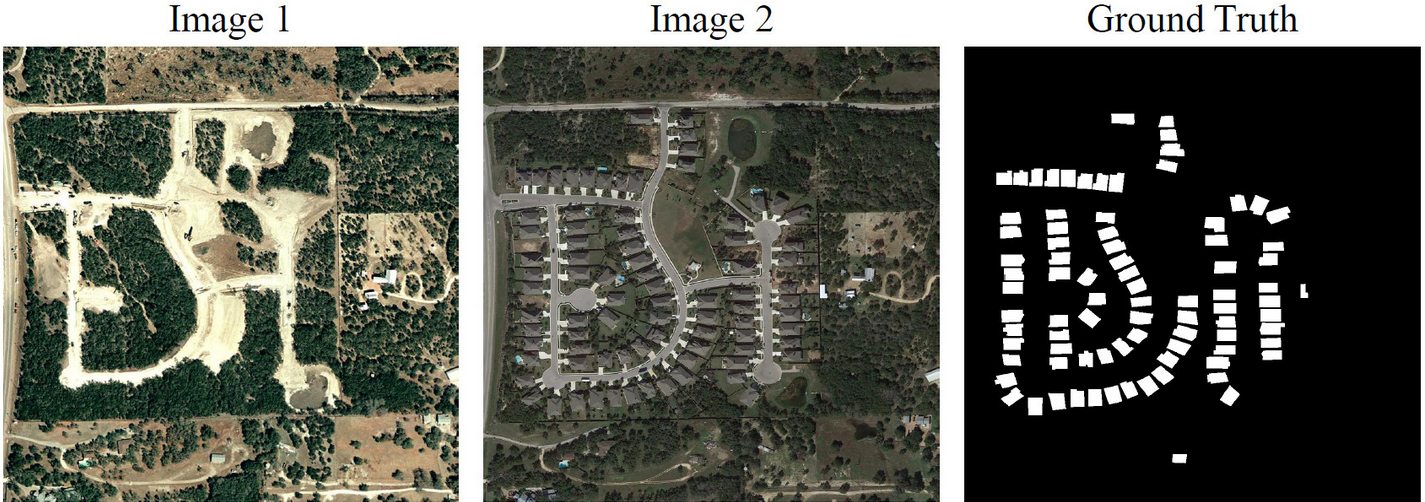
\includegraphics[width=0.6\textwidth]{graficos/LevirCD2.png}
    \caption{Building Change Detection - Levir CD Dataset sample. In this sample it comperes two images and detect only the buildings has changed in determined time. \cite{Zheng2020LEVIR}}
    \label{fig:LevirCD2}
\end{figure}

\subsection{The Change Detection Problem}

There are several challenges that make the building change detection problem particularly complex. First, changes may be subtle or gradual, such as vertical densification, where the spectral signature of a building does not change significantly, but its height does\cite{Cheng2021DeepLab}. Second, the precise registration of images from different dates is often imprecise, introducing geometric misalignment that can be mistaken as change. Third, satellite images contain noise due to clouds, shadows, or atmospheric conditions, which obscure true variations. Finally, and most critically, the scarcity of reliable labeled datasets at very high resolution (VHR) for Latin American cities limits the training and validation of deep learning models.

\begin{figure}[h!]
    \centering
    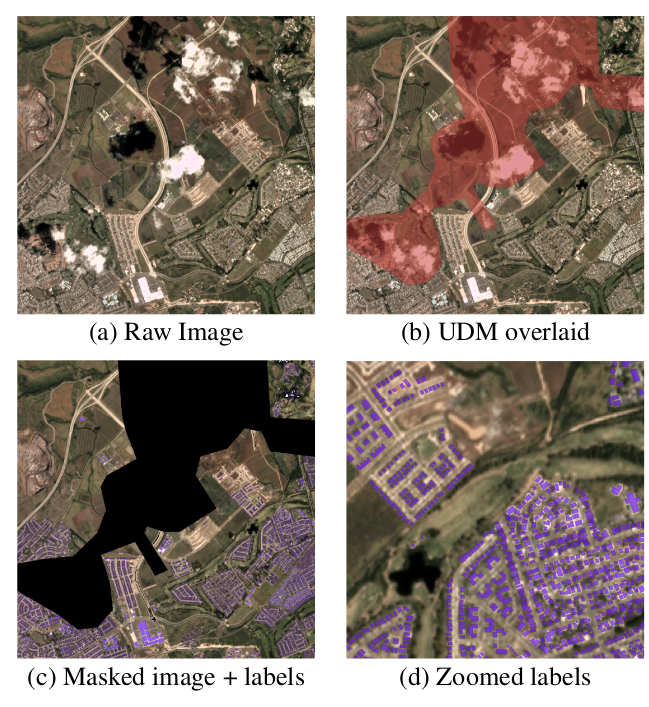
\includegraphics[width=0.6\textwidth]{graficos/spacenet7.png}
    \caption{Building Change Detection - SpaceNet 7 Dataset sample. In this sample we can see the process of remove clouds and recovery the complete view of the satellital image. \cite{VanEtten2021SpaceNet}}
    \label{fig:LevirCD2}
\end{figure}

From this perspective, the building change detection process must consider several aspects: the nature of the input data (VHR vs. medium-resolution), the type of change to be detected (footprint vs. height), the availability of annotated labels (manual vs. crowdsourced), and the expected output (binary masks, change maps, or height proxies). Each of these elements strongly conditions the accuracy and generalization of the models.

\newpage

\subsection{Types of Changes in Urban Environments} 

Building changes can be broadly classified into three categories:

\noindent \textbf{Horizontal expansion}: the appearance of new building footprints in previously unoccupied land\cite{Zheng2020LEVIR}.

\noindent \textbf{Vertical densification}: the increase in the number of floors or average building height, often without a change in footprint\cite{Cheng2021DeepLab}.

\noindent \textbf{Functional or material change}: modifications in the use or structure of a building (e.g., reconstruction, demolition, or replacement), less studied but relevant in resilience analysis.

\newpage 

\begin{figure}[h!]
    \centering
    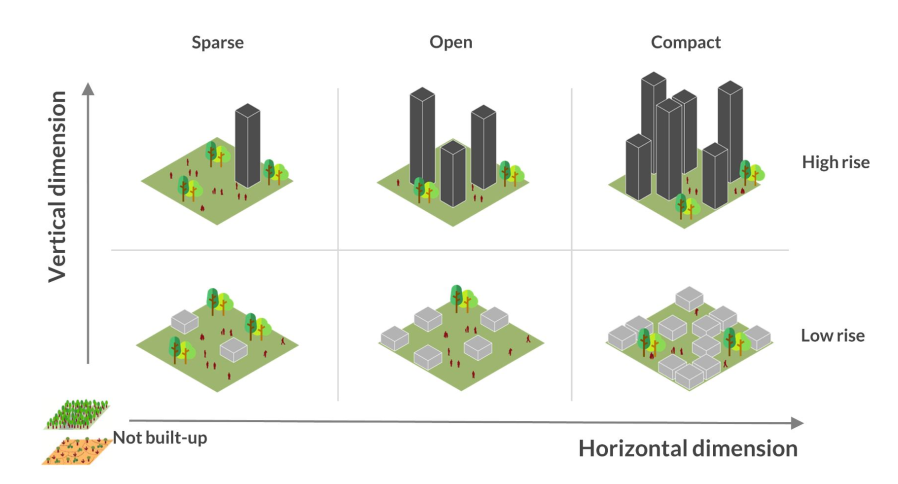
\includegraphics[width=0.6\textwidth]{graficos/hor-vert.png}
    \caption{Classification schema for urban density in horizontal and vertical dimensions. \cite{Cheng2021DeepLab}}
    \label{fig:LevirCD2}
\end{figure}

Horizontal changes are easier to detect in satellite imagery, since they involve new shapes and edges in the spatial domain. In contrast, vertical changes require proxies such as shadows, stereo imagery, or contextual socio-economic data, which increases the computational and methodological complexity\cite{Sirko2023TeachStudentSentinel2}.

\subsection{Approaches to Building Change Detection}
\label{subsec:approaches-bcd}

Depending on the availability and quality of labels, building change detection can be addressed through three main paradigms: \emph{supervised}, \emph{semi-supervised}, and \emph{self-supervised} learning. Each setup imposes different assumptions on data annotation and provides distinct trade-offs in terms of accuracy, robustness to noise, and scalability across geographies and sensors.

\label{subsubsec:supervised-bcd}
\noindent \textbf{Supervised Building Change Detection.} The training set comprises fully labeled pairs (or sequences) of multi-temporal images with ground-truth change masks. A change detector is trained end-to-end to predict per-pixel labels (change / no-change), closely mirroring traditional semantic segmentation with a temporal dimension. Typical outputs are \emph{binary change maps} and per-pixel confidence scores.

\begin{figure}[h!]
    \centering
    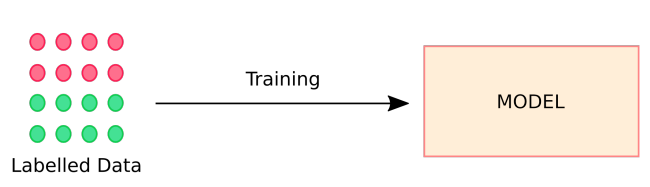
\includegraphics[width=0.6\textwidth]{graficos/supervised.png}
    \caption{Supervised building change detection illustration.}
    \label{fig:LevirCD2}
\end{figure}

In remote sensing, early methods include CNN-based siamese architectures with attention and dense connections to preserve edges and multi-scale context (e.g., STANet and SNUNet-CD), while more recent approaches leverage Transformers (e.g., BIT and ChangeFormer) to capture long-range spatial-temporal dependencies and improve performance with fewer parameters \cite{Zheng2020LEVIR,Fang2021SNUNetCD,Chen2022BIT,Bandara2022ChangeFormer}. These models achieve strong results on benchmarks such as LEVIR-CD but require large, clean, and well-registered labeled datasets; geometric misalignment and label scarcity can substantially degrade performance.

\label{subsubsec:semisupervised-bcd}
\noindent \textbf{Semi-Supervised Building Change Detection.} Assumes a small amount of labeled data together with a larger pool of unlabeled or weakly-labeled samples. The model exploits \emph{consistency regularization}, \emph{pseudo-labeling}, or \emph{teacher--student} schemes to transfer supervision from labeled to unlabeled data. Outputs remain \emph{pixel-wise change masks}, often accompanied by uncertainty or confidence estimates for pseudo-label filtering.

\begin{figure}[h!]
    \centering
    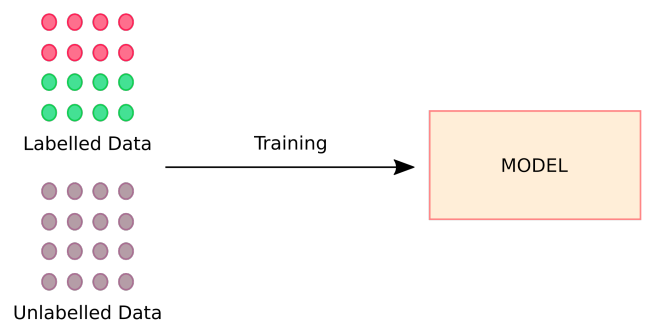
\includegraphics[width=0.6\textwidth]{graficos/semisupervised.png}
    \caption{Semi-supervsied building change detection illustration.}
    \label{fig:LevirCD2}
\end{figure}

In the building domain, semi-supervised strategies have been used to \emph{update} or \emph{refine} building footprints and change masks with limited labels, showing that high accuracy can be reached even when using only a fraction of annotations, provided that a high-quality prior or auxiliary map is available (e.g., SG-EPUNet) \cite{Guo2021SGEPUNet}. Likewise, cross-task transfer from \emph{crowdsourced} maps such as OSM can be effective when robust to label noise (e.g., FFCTL), though performance depends on the completeness and positional accuracy of the external source \cite{Cao2023FFCTL}. Data generation techniques such as ISPG (GAN-based) augment scarce bi-temporal pairs, improving IoU/F1 on standard benchmarks; however, synthetic samples may induce unrealistic biases if not carefully curated \cite{Li2023ISPG}.

\label{subsubsec:selfsupervised-bcd}
\noindent \textbf{Self-Supervised Building Change Detection.} Minimizes (self-supervised) the dependency on manual labels. The model learns from intrinsic data structure by solving \emph{pretext tasks} such as masked reconstruction (MAE) or contrastive alignment across time, scale, and spectral bands. The outputs can be \emph{change scores} (later thresholded) or change masks obtained after a light supervised fine-tuning stage.

\newpage

\begin{figure}[h!]
    \centering
    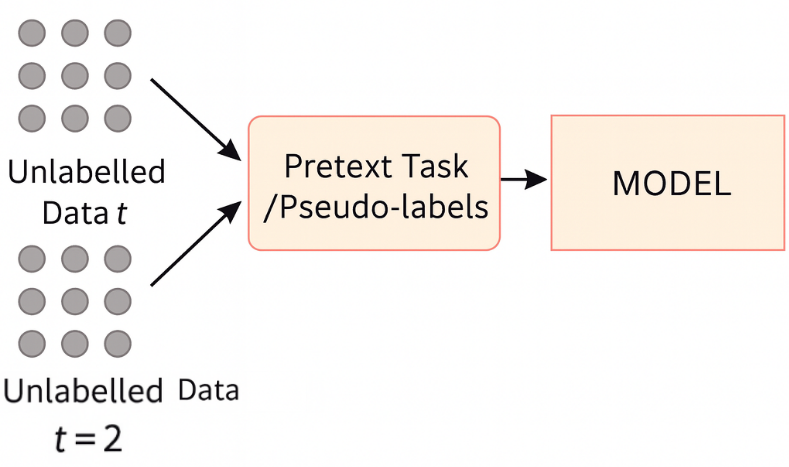
\includegraphics[width=0.6\textwidth]{graficos/selfsupervised.png}
    \caption{Self-supervised building change detection.}
    \label{fig:LevirCD2}
\end{figure}

Masked Autoencoders (MAE) learn rich visual representations by reconstructing heavily masked inputs and have proven scalable in vision \cite{He2022MAE}. Their adaptations to Earth Observation, such as SatMAE and Cross-Scale MAE, incorporate temporal and multi-spectral tokens (Sentinel/Landsat) and enforce cross-scale coherence to enhance transfer across resolutions \cite{Cong2022SatMAE,Tang2023CrossScaleMAE}. In bi-temporal scenarios, a siamese encoder with temporal contrastive loss can enforce invariance across dates for static background while preserving sensitivity to structural changes, enabling downstream change detection with minimal labels. This paradigm is particularly suitable in Very High Resolution (VHR) contexts where manual labeling is costly and crowdsourced maps are noisy or incomplete.

\begin{figure}[h!]
    \centering
    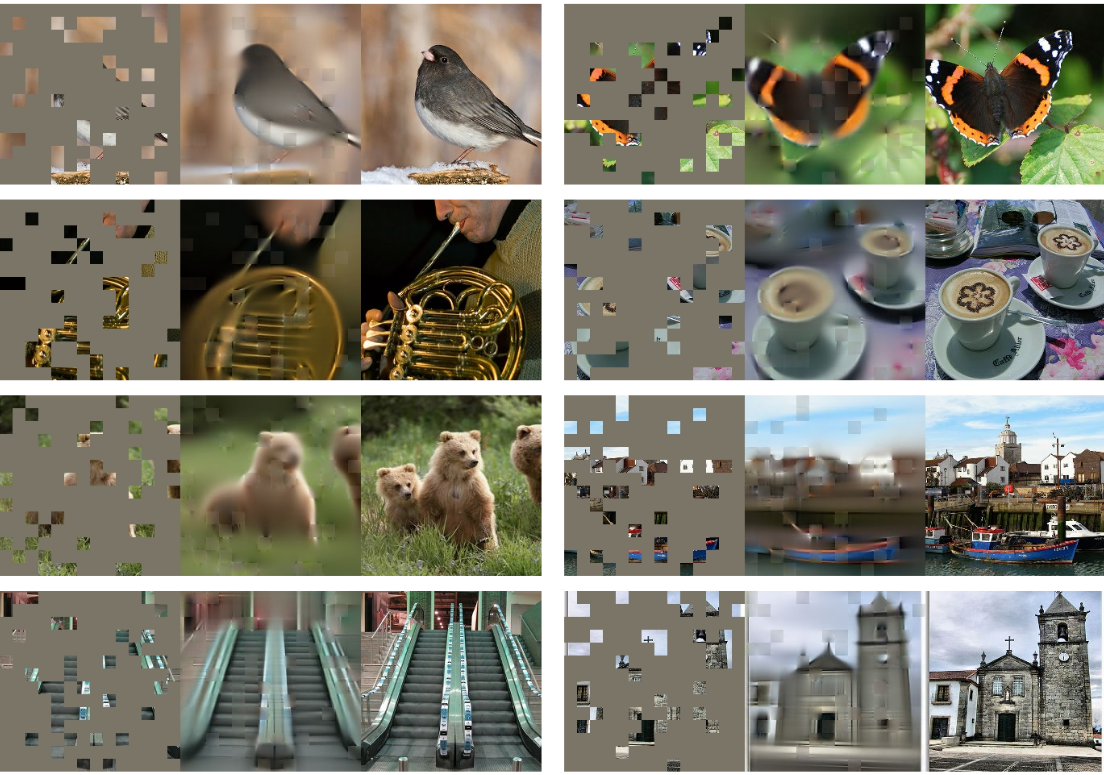
\includegraphics[width=0.6\textwidth]{graficos/MAE.png}
    \caption{Results of reconstructed images from different domains using Masked Autoencoder (MAE). \cite{He2022MAE}}
    \label{fig:LevirCD2}
\end{figure}

\medskip
\noindent
Labeling each building footprint across thousands of PeruSAT-1 VHR tiles is infeasible, and crowdsourced sources such as OpenStreetMap contain omissions and positional errors. In this setting, self-supervised learning provides a principled route to reduce label dependence while preserving performance, which motivates the adoption of MAE-based pretraining and temporal contrastive alignment in this research.

\section{Transformers and Attention for BCD}
\label{sec:transformers-attn}

Transformer-based models have reshaped building change detection by capturing long-range spatial-temporal dependencies across multi-temporal inputs. This section introduces the standard self-attention mechanism, highlights its computational bottlenecks on VHR imagery, and presents linear/low-rank attention approximations with emphasis on Reduced-Rank Linear Attention (RALA) as an efficiency enabler for the change detection backbone.

\subsection{Self-Attention (Softmax) and Quadratic Complexity}
\label{subsec:softmax-attn}

\noindent Let an image be divided into $N$ patches $\{\mathbf{x}_i\}_{i=1}^N$ embedded into $\mathbf{X}\in\mathbb{R}^{N\times d}$. A Transformer layer computes:
\begin{equation}
\mathbf{Q} = \mathbf{X}\mathbf{W}_Q,\quad
\mathbf{K} = \mathbf{X}\mathbf{W}_K,\quad
\mathbf{V} = \mathbf{X}\mathbf{W}_V,\quad \mathbf{W}_{\{\cdot\}}\in\mathbb{R}^{d\times d_k}.
\end{equation}
Scaled dot-product attention \cite{Vaswani2017Attention} is
\begin{equation}
\label{eq:softmax-attn}
\mathrm{Attn}(\mathbf{Q},\mathbf{K},\mathbf{V}) = \mathrm{softmax}\!\left(\frac{\mathbf{Q}\mathbf{K}^{\top}}{\sqrt{d_k}}\right)\mathbf{V}.
\end{equation}
This requires computing the dense matrix $\mathbf{Q}\mathbf{K}^{\top}\in\mathbb{R}^{N\times N}$, leading to $\mathcal{O}(N^2)$ memory and time, which becomes prohibitive for large $N$ (e.g., VHR $1024\times 1024$ images patchified at small patch sizes, or multi-scale tokens).

\begin{figure}[h!]
    \centering
    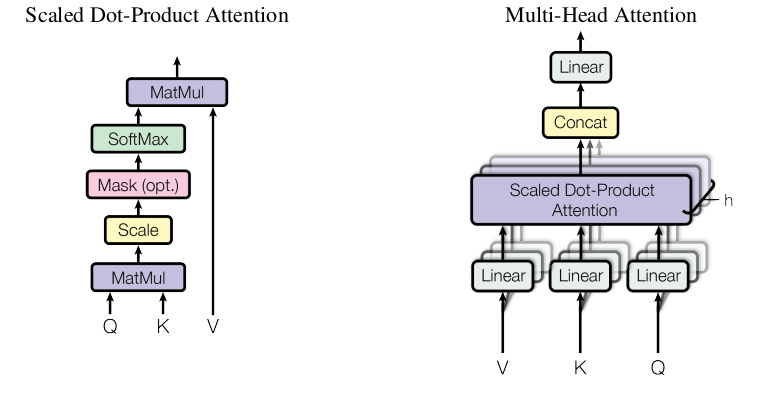
\includegraphics[width=0.6\textwidth]{graficos/MHSA.png}
    \caption{Scaled dot-product attention (left) and Multi-Head Self-Attention (right). MHSA applies several attention heads in parallel \cite{Vaswani2017Attention}.}
    \label{fig:mhsa}
\end{figure}

% ============================================================
\subsection{From Softmax to Linear Attention}
\label{subsec:linear-attn}
% ============================================================

\noindent Given a sequence of tokens $X = [x_1,\dots,x_N]$, standard self–attention computes
\begin{equation}
\mathrm{Attn}(Q,K,V)
   = \mathrm{softmax}\!\left(\frac{QK^\top}{\sqrt{d}}\right)V,
\end{equation}
where $Q,K,V \in \mathbb{R}^{N \times d}$ and the resulting affinity matrix
$QK^\top \in \mathbb{R}^{N \times N}$ yields the well–known
$\mathcal{O}(N^2)$ complexity.

\noindent Linear attention replaces the softmax kernel with a positive kernel map
$\kappa(\cdot)$ and changes the computation order:
\begin{equation}
\label{eq:lin-attn}
Y_i
= \frac{\kappa(Q_i) \big( \sum_{j=1}^{N} \kappa(K_j)^{\top} V_j \big)}
       {\kappa(Q_i) \big( \sum_{m=1}^{N} \kappa(K_m)^{\top} \mathbf{1} \big)}.
\end{equation}

\noindent This decomposes the quadratic term $QK^\top$ into  
a kernel-feature product and a global \emph{KV buffer},
\[
B_\text{lin} = \sum_{j=1}^{N} \kappa(K_j)^\top V_j \in \mathbb{R}^{d \times d},
\]
reducing complexity to $\mathcal{O}(Nd)$.

\noindent However, as proved in \cite{Fan2025RALA}, the KV buffer and the
resulting output features  
\[
Y = \kappa(Q)\, B_\text{lin}
\]
exhibit \textbf{significant rank collapse}, typically
$\mathrm{Rank}(Y) \ll d$, severely limiting spatial modeling power.


% ============================================================
\subsection{Rank-Augmented Linear Attention (RALA)}
\label{subsec:rala}
% ============================================================

\noindent RALA \cite{Fan2025RALA} identifies \textbf{two independent sources of
low-rank degeneration} in linear attention: (a) the KV buffer $B_\text{lin}$ is intrinsically low-rank,  (b) even a full–rank KV buffer yields a low-rank output $Y$ due to $\mathrm{Rank}(\kappa(Q) B) \le \min(\mathrm{Rank}(\kappa(Q)),\mathrm{Rank}(B))$. RALA resolves both problems via:

\textbf{1. Rank augmentation of the KV buffer}

\noindent Instead of treating each token equally, RALA reweights each
key–value pair according to a \textbf{context-aware coefficient}
$\alpha_j$:
\begin{equation}
\label{eq:rala-buffer}
B
= \sum_{j=1}^{N} \alpha_j\, \kappa(K_j)^\top V_j,
\qquad 
\sum_{j=1}^{N} \alpha_j = N.
\end{equation}

\noindent \textbf{Global query for token importance} A global query summarizes global content:
\begin{equation}
Q_g = \frac{1}{N}\sum_{i=1}^{N} Q_i.
\end{equation}

\noindent The importance of token $j$ is measured through a kernel similarity:
\begin{equation}
\label{eq:alpha}
\alpha_j
= N \cdot 
\frac{\exp\big( \kappa(Q_g)\kappa(K_j)^\top \big)}
     {\sum_{m=1}^{N} \exp\big( \kappa(Q_g)\kappa(K_m)^\top \big)}.
\end{equation}

\noindent This modulates the KV buffer using a \textbf{softmax-like redistribution} of information content.

\paragraph{Effect.}  
Weighting different rank-1 matrices $\kappa(K_j)^\top V_j$ differently
creates a \textbf{sum of non-collinear matrices} provably increasing matrix
rank (Appendix A, \cite{Fan2025RALA}):
\[
\mathrm{Rank}\!\left( \sum_j \alpha_j u_j v_j^\top \right)
    \;\text{grows with token diversity}.
\]

\textbf{2. Rank restoration in the output features}

\noindent Even if $B$ is full-rank, the output
\(
Y = \kappa(Q)\, B
\)
remains low-rank because all rows are linear combinations of the
same $d$-dimensional basis.

\noindent RALA fixes this by modulating each output token with its own
input-dependent channel-wise correction:
\begin{equation}
\label{eq:rala-out}
Y_i
   = \phi(X_i) \odot
     \Big( \kappa(Q_i)\, B \Big),
\end{equation}
\noindent where $\phi(\cdot)$ is a learnable projection
and $\odot$ denotes the Hadamard product.

\noindent This injects token-specific structure and restores the diversity of
$Y$, as experimentally shown in Fig. 5 of \cite{Fan2025RALA}.

\noindent \textbf{Final RALA Attention}

\noindent Combining (\ref{eq:rala-buffer})–(\ref{eq:rala-out}), RALA computes:
\begin{align}
B &= \sum_{j=1}^N \alpha_j\, \kappa(K_j)^\top V_j,
\\[4pt]
Y_i &= 
\phi(X_i) \odot 
\Big( 
  \kappa(Q_i)\, B
\Big).
\end{align}

\noindent \textbf{Complexity}
RALA preserves the linear cost of kernel attention:
\[
\mathcal{O}(N d),
\]
\noindent while producing \textbf{full-rank feature maps comparable to Softmax attention}.

\paragraph{Loss function.}  
For building-change detection, all variants of ChangeFormer and RALA use
Binary Cross-Entropy (BCE) loss:
\[
\mathcal{L}_\text{BCE}
 = -\big( y \log \hat{y} + (1-y)\log(1-\hat{y}) \big).
\]

\newpage

% ============================================================
\subsection{Integration into ChangeFormer}
\label{subsec:rala-cf}
% ============================================================

\noindent ChangeFormer processes bi-temporal features  
$F^{(l)}_{t_1}, F^{(l)}_{t_2}$ through Transformer blocks containing MHSA.
We replace each MHSA block with a RALA block:

\begin{equation}
X^{(l)} =
\mathrm{PatchEmbed}(F^{(l)}_{t_1})
\;\Vert\;
\mathrm{PatchEmbed}(F^{(l)}_{t_2}),
\end{equation}
\[
X^{(l)} \;\xrightarrow{\;\text{RALA block}\;}
X^{(l)}_{\text{out}}.
\]

\noindent Since RALA is drop-in compatible with MHSA and preserves global
contextual aggregation, the overall architecture remains unchanged,
but: (i) memory usage drops significantly,  (ii) FLOPs decrease and (iii) larger batch sizes and higher-resolution patches become feasible.

\noindent This allows RALA-ChangeFormer to operate efficiently on large
bi-temporal remote sensing patches typical of VHR datasets such as
LEVIR-CD and DSIFN-CD.

\noindent \textbf{Implications for Change Detection Backbones}
\label{subsec:rala-for-bcd}

\noindent Change detection backbones such as \textbf{ChangeFormer} \cite{Bandara2022ChangeFormer} leverage Siamese encoders and cross-temporal fusion using Transformer blocks. However, standard MHSA incurs $\mathcal{O}(N^2)$ complexity with respect to sequence length (number of patches), which is costly for VHR imagery and multi-scale hierarchies. By replacing MHSA with \textbf{RALA} layers, we can (i) reduce attention complexity from quadratic to near-linear in $N$, (ii) lower GPU memory usage, enabling larger batch sizes or higher input resolutions and (iii) maintain global context modeling through the recurrent low-rank state $\mathbf{S}_t$.

Section~\ref{sec:enablers-transformers} of Chapter~3 already positioned Transformers and attention variants as key enablers, here we provide the mathematical underpinnings that justify the \textbf{model} design adopted in Chapter~4.


\section{Performance Metrics}
\label{sec:metrics}

This section introduces the evaluation metrics employed to validate the performance of the proposed model and baselines in building change detection. Since the task is formulated as a semantic segmentation problem over very high resolution imagery, the evaluation focuses on overlap-based metrics and class-specific scores under class imbalance.

\noindent \textbf{Intersection over Union (IoU).} Intersection over Union, also known as the Jaccard index, is the most common metric for semantic segmentation. It is defined as the ratio between the area of intersection and the area of union of the predicted mask $P$ and the ground truth mask $G$. For the building change detection task, IoU is computed at the pixel level as:
\begin{equation}
IoU = \frac{|P \cap G|}{|P \cup G|}
\end{equation}
Higher IoU indicates that the predicted footprints or change masks align more closely with the reference annotations. This metric is sensitive to both false positives and false negatives, making it particularly relevant when boundaries of buildings must be preserved.

\noindent \textbf{F1-Score (Dice Coefficient).} The F1-score, also known as the Dice coefficient, provides a harmonic mean of precision and recall. It is particularly useful in binary segmentation where the positive class (buildings or changes) is much smaller than the background:
\begin{equation}
F1 = \frac{2 \cdot TP}{2 \cdot TP + FP + FN}
\end{equation}
where $TP$, $FP$, and $FN$ denote true positives, false positives, and false negatives, respectively. F1 is more robust than accuracy in highly imbalanced datasets, since it focuses on the correct detection of the minority class (changed buildings).

\noindent \textbf{Precision–Recall Curve and AUC.} In scenarios with severe class imbalance---where the majority of pixels correspond to unchanged background---the Precision–Recall (PR) curve provides a more informative picture than the Receiver Operating Characteristic (ROC) curve. Precision measures the fraction of predicted positives that are correct, while recall measures the fraction of actual positives that are retrieved. By plotting precision against recall for different thresholds, the PR curve highlights the trade-off between false alarms and missed detections. 

The Area Under the Precision–Recall Curve (AUC-PR) is used as a scalar summary of performance:
\begin{equation}
AUC\text{-}PR = \int_0^1 Precision(Recall) \, d(Recall)
\end{equation}
A higher AUC-PR indicates that the model maintains high precision even as recall increases, which is desirable when detecting sparse changes in dense urban imagery.

\noindent \textbf{Considerations for Class Imbalance.} In building change detection, the proportion of pixels belonging to the ``change'' class is typically much smaller than that of the background. Metrics such as accuracy or even ROC-AUC can be misleading in this setting, as they may overestimate performance by favoring the dominant class. For this reason, IoU, F1-score, and AUC-PR are prioritized in this research.

\begin{figure}[h!]
    \centering
    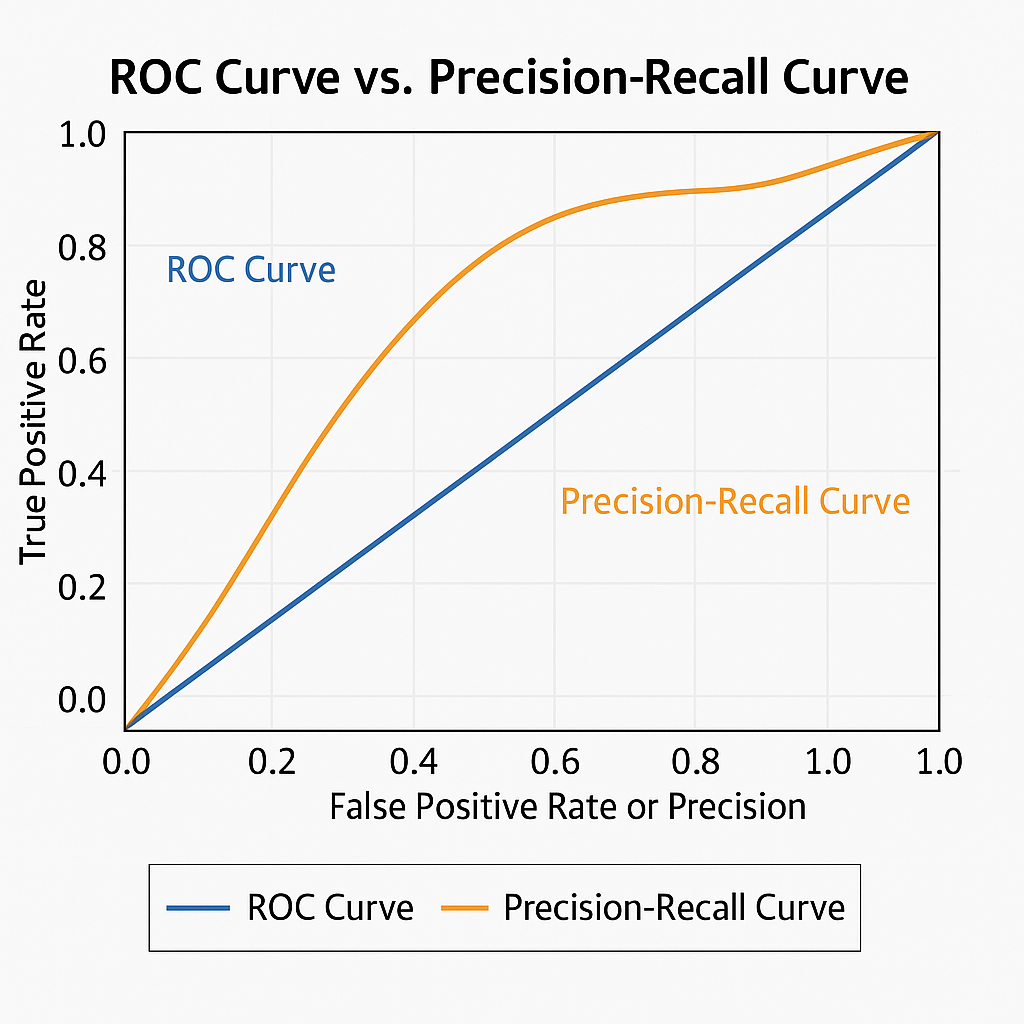
\includegraphics[width=0.6\textwidth]{graficos/ROCvsPC.png}
    \caption{ROC curve vs PR curve trade-off for imbalanced classes.}
    \label{fig:LevirCD2}
\end{figure}

\newpage

\section{Final Considerations}
\label{sec:bg-final}

This chapter established the conceptual and computational foundations for efficient multi-temporal building change detection (BCD) on Very High Resolution (VHR) imagery. From the remote sensing standpoint, systems such as PeruSAT-1 enable building-level analysis but also induce large sequence lengths once images are patchified, elevating memory and time costs in Transformer-based models. From the modeling standpoint, while backbones like ChangeFormer effectively capture long-range spatio-temporal context, their reliance on standard multi-head self-attention entails \(\mathcal{O}(N^2)\) complexity with respect to the number of tokens.

To address these constraints, we reviewed linear/low-rank attention mechanisms and detailed the Reduced-Rank Linear Attention (RALA) formulation. RALA summarizes key–value interactions via a recurrent low-rank state, enabling attention to scale near-linearly in sequence length and reducing GPU memory consumption. This property is particularly relevant for VHR imagery and bi-temporal pipelines, where the number of tokens grows quickly with input resolution and multi-scale representations.

In parallel, we revisited the learning regimes used in BCD (supervised, semi-supervised, and self-/unsupervised). Although supervised approaches dominate performance in standard benchmarks (e.g., LEVIR-CD, DSIFN-CD), their annotation requirements are often a bottleneck in Latin American settings. Self-supervised learning (SSL)thus remains a complementary tool: optional MAE-style reconstruction or temporal contrastive pretraining can be incorporated to improve the backbone’s representation quality under scarce or noisy labels. Nevertheless, the central thrust of this thesis is computational: \textbf{integrating RALA into ChangeFormer} to lower the cost of attention without sacrificing accuracy.

Finally, we outlined the evaluation perspective tailored to imbalanced, pixel-wise change detection tasks, emphasizing IoU, F1-score, and AUC-PR over accuracy-based summaries. These metrics better reflect model behavior on sparse building changes against dominant background classes.

\textbf{Bridge to the next chapters.} The next chapters instantiate these ideas into a concrete architecture and training pipeline: we (i) integrate \textbf{RALA} into the Transformer blocks of \textbf{ChangeFormer}, (ii) adopt a practical preprocessing and patching scheme for \textbf{LEVIR-CD} and \textbf{DSIFN-CD}, and (iii) prepare the incorporation of \textbf{PeruSAT-1} VHR tiles. We then quantify the trade-offs between accuracy and efficiency, showing that RALA-augmented attention reduces computational overhead while preserving— and in some cases improving— downstream change detection performance.

